\documentclass{article}

\usepackage{amsmath, amsthm, amssymb, amsfonts}
\usepackage{thmtools}
\usepackage{graphicx}
\usepackage{setspace}
\usepackage{geometry}
\usepackage{float}
\usepackage{hyperref}
\usepackage[utf8]{inputenc}
\usepackage[english]{babel}
\usepackage{framed}
\usepackage[dvipsnames]{xcolor}
\usepackage[most]{tcolorbox}
\usepackage{minted}
\usepackage{enumitem}

\usepackage{indentfirst}

\usepackage[export]{adjustbox} % Align images

\colorlet{LightGray}{White!90!Periwinkle}
\colorlet{LightOrange}{Orange!15}
\colorlet{LightGreen}{Green!15}

\newcommand{\HRule}[1]{\rule{\linewidth}{#1}}

\newtcbtheorem[auto counter,number within=section]{code}{Código}{
  colback=LightOrange!20,
  colframe=LightOrange,
  colbacktitle=LightOrange,
  fonttitle=\bfseries\color{black},
  boxed title style={size=small,colframe=LightOrange},
}{code}

\setstretch{1.2}
\geometry{
  textheight=22.5cm,
  textwidth=13.75cm,
  top=2.5cm,
  headheight=12pt,
  headsep=25pt,
  footskip=30pt
}

% ------------------------------------------------------------------------------


\begin{document}
\maketitle

\section{Introduction}
This report presents an analysis of the breast cancer dataset using a combination of EM clustering, logistic regression, and Radial Basis Function (RBF) networks. 

\section{Methodology}
\subsection{Clustering}
We utilized scikit-learn's gaussian mixture model to perform Expectation-Maximization (EM) clustering on the breast cancer dataset features. 
The quality of clustering was evaluated using the Silhouette score for different values of k: 

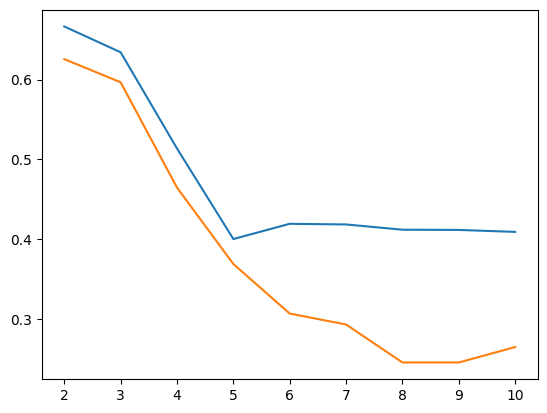
\includegraphics[width=10cm]{img/silhouttes.png}

According to the results obtained the optimal k is k=2 with a train silhouette score of 0.667 and a test silhouette score of 0.626

\section{Results and Analysis}
\subsection{Baseline Performance}
Upon fitting a logistic regression on the breast cancer dataset we obtained a train accuracy of 0.960 and a test accuracy of 0.977. 

\subsection{Clustering-Based Classification}
Using k=2 clusters (the optimal value determined through Silhouette analysis), we mapped the dataset to their cluster probabilities and performed logistic regression on these transformed features. 

This procedure uses EM clustering as a dimensionality reduction technique, reducing the feature space from 30 features to 2 features. 

This result demonstrates the effectiveness of using cluster probabilities as features for classification, and therefore EM clustering proves as an effective dimensionality reduction on the dataset. This also reinforces that there is high cluster quality with these 2 clusters. 

\section{RBF Network Implementation}
\subsection{Theoretical Background}
According to Wikipedia\footnote{\url{https://en.wikipedia.org/wiki/Radial_basis_function_network}}, "Radial basis function (RBF) networks typically have three layers: an input layer, a hidden layer with a non-linear RBF activation function and a linear output layer." The same source describes the operational procedure: "An input vector x is used as input to all radial basis functions, each with different parameters. The output of the network is a linear combination of the outputs from radial basis functions."

The rbf network processes input vectors through multiple radial basis functions in the hidden layer. The final output is computed as a linear combination of these RBF outputs. This architecture can be represented mathematically as:

In our implementation, following [Reference]\cite{rbf_reference}, we utilized the Mahalanobis distance metric in conjunction with the EM clustering results, as this distance measure naturally aligns with the parameters produced from EM clustering. To create the RBF network architecture, our approach consists of two main steps:

\begin{enumerate}
    \item Feature Transformation: Transform the original features using RBF functions based on Mahalanobis distances to cluster centers, effectively implementing the hidden layer's non-linear transformations
    \item Linear Classification: Apply logistic regression to these transformed features, representing the linear output layer of the network
\end{enumerate}

\subsection{RBF Transformations}
Two different RBF transformations were implemented:
\begin{enumerate}
    \item Gaussian RBF: $\phi(x) = exp(-0.5 * d(x))$, where d(x) is the Mahalanobis distance
    \item Linear RBF: $\phi(x) = d(x)$
\end{enumerate}

Both approaches are valid as RBF transformations since they maintain the fundamental principle of mapping inputs based on their distance to cluster centers. The key requirement for RBF is that the transformation is a function of the distance between points, which both implementations satisfy.
    
\section{Comparative Analysis}
The different approaches yielded varying results:
\begin{itemize}
    \item Baseline Logistic Regression: train accuracy = 96.0\%; test accuracy = 97.7\%
    \item Logistic regression on transformed features (k=2): 92.4\%
    \item Gaussian RBF Network: 89.1\%
    \item Linear RBF Network: 91.7\%
\end{itemize}

Explanation % TODO

\section{Conclusion}
The study demonstrates the effectiveness of using clustering as a dimensionality reduction technique, successfully reducing the feature space from 30 dimensions to just 2 while maintaining high classification accuracy. The high performance of the cluster probability approach (92.4\%) suggests that the EM clustering effectively captured the underlying structure of the data.

\bibliographystyle{plain}
\bibliography{references}

\end{document}